% oja_template.tex
% Unofficial LaTeX template for publishing 
% in the Open Journal of Astrophysics
% v1.0 released September 6, 2015 (matches openjournal.cls)
% Author: Emmanuel Frion

% Basic setup
\documentclass[12pt]{openjournal}
% Available options:
% [twocolumn] - two-column mode
% [onecolumn] - (default) main text in one-column mode
% [apj]       - typeset in the style of ApJ.
% [apjl]      - (default) typeset in the style of ApJ Letters 
% [tighten]   - some adjustments to approximate grid typesetting
% [numberedappendix]   - number appendix sections as A, B, etc
% [appendixfloats]  - use separate numbering for floats within appendix
% [twocolappendix]  - make appendix in two-col mode in a two-col paper
% [revtex4]   - force using revtex4 (rather than 4-1)

% Remove this package
\usepackage{lipsum}

% Optional useful packages
\usepackage{xcolor}
\usepackage{textgreek}
\usepackage[utf8]{inputenc}
\usepackage[english]{babel}
\usepackage{hyperref}
\hypersetup{
    colorlinks=true,
    linkcolor=blue,
    filecolor=blue,      
    urlcolor=red,
    citecolor=blue,
}
\usepackage{color,colortbl}
\usepackage{tensind}
\tensordelimiter{?}
\DeclareGraphicsExtensions{.bmp,.png,.jpg,.pdf}
\usepackage{verbatim}
\usepackage[normalem]{ulem}
\usepackage{orcidlink}
\usepackage{soul}

\urlstyle{same}

% Define path to put your plots, figures, etc...
\graphicspath{ {./figs/} }

\begin{document}
\title{Your awesome paper}


\author{Author 1\orcidlink{0000-0000-0000-0000}}
\email{author1@you.com}
\affiliation{Your nice institute / university}
\affiliation{Your second nice institute / university}

\author{Author 2\orcidlink{0000-0000-0000-0000}}
\email{author2@you.com}
\affiliation{Your nice institute / university}
\affiliation{Your second nice institute / university}



\begin{abstract}
    What's your paper about?
    \lipsum[50]
\end{abstract}

% Write your keywords here
\begin{keywords}
    {First, second}
\end{keywords}

\maketitle


\section{Introduction}
\label{sec:intro}

The Universe is awesome and deserves to be studied \cite{me}.

\lipsum[10]


\section{Section}
\label{sec:sec}

\lipsum[12]

\subsection{Subsection  (\texorpdfstring{$ H_0 $}{})}

% Write your own, nice-looking table
\begingroup % Optional: affects only this particular table
    \setlength{\tabcolsep}{10pt} % Default value: 6pt
    \renewcommand{\arraystretch}{1.5} % Default value: 1
    \begin{table}
        \centering
        \begin{tabular}{ c c }  
            Parameter & Prior \\
            \hline \hline     
            {\boldmath$\alpha$} & $\left[ 10^{-3}, 10 \right]$ \\
            {\boldmath$\beta$} & $\left[ 0, 1 \right]$ \\   
            \hline \hline  
        \end{tabular}  
        \caption{Parameters used in your paper.}
        \label{table:table}
    \end{table}
\endgroup

Refer to your nice table (Table~\ref{table:table}).


\lipsum[14]

\begin{center}
    \begin{figure}[!t]
        \centering
    	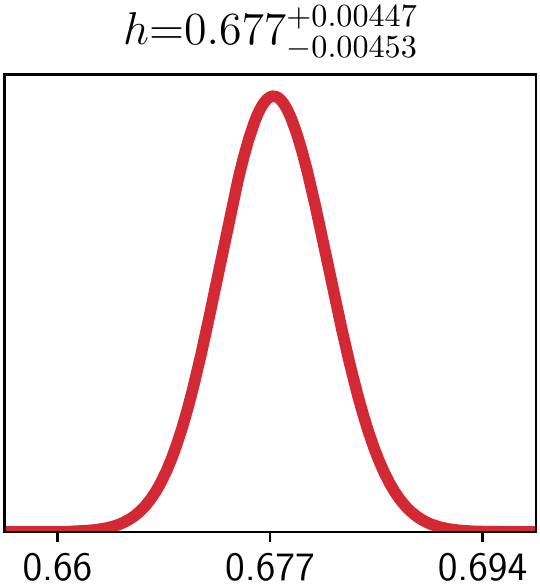
\includegraphics[scale=0.3]{figs/probdist.png}
    	\caption{Nice plot. \lipsum[11]}
        \label{fig:fig}
    \end{figure}
\end{center}


Refer to your nice figure (Fig.~\ref{fig:fig}).

\section{Discussion}
\label{sec:concl}


We find that  \lipsum[6]



\section*{Acknowledgments}

Acknowledge support (or not).

\bibliographystyle{apsrev4-1}

% You should give the same name for your .bbl as your main .tex
% since it is a requirement for posting on ArXiv.
\bibliography{oja_template}


\begin{appendix}

\section{Appendix 1}
\label{ap:ap}
\lipsum[4]

\end{appendix}


 

\end{document}
